\section{Time integration}

\subsection{Strang splitting method}

Consider the Cauhcy problem

\begin{equation}
    \begin{cases}
        \pdv{u}{t} = (A + B) u \\
        u(0) = u_0
    \end{cases}
    \label{eq:cauchy}
\end{equation}

\begin{proposition}
    If $A$ and $B$ commute, then $\exp(A+B) = \exp(A)\exp(B)$
\end{proposition}

\begin{proof}
    
    \begin{align*}
        \exp(A + B) &= \sum_{n = 0}^\infty \frac{(A + B)^n}{n!} \\
                    &= \sum_{n = 0}^\infty \sum_{k = 0}^n \binom{n}{k} \frac{A^k B^{n-k}}{n!} \\
                    &= \sum_{n = 0}^\infty \sum_{k = 0}^n \frac{A^k}{k!} \frac{B^{n - k}}{(n - k)!}  \quad \ell = n - k \\
                    &= \sum_{k = 0}^\infty \frac{A^k}{k!} \sum_{\ell = 0}^\infty \frac{B^\ell}{\ell!} \\
                    &= \exp(A)\exp(B)
    \end{align*}

\end{proof}

The analytical solution for \ref{eq:cauchy} is

\[ u(t) = e^{(A + B)t} u_0 \]

So, for the previous proposition, if $A$ and $B$ commute, then $u(t) = e^{tA}e^{tB}u_0 \implies u(t + \tau) = e^{\tau A}e^{\tau B}u(t)$.

This is equivalent to solve separately two initial value problems:

\[
    \begin{cases}
        \pdv{u}{t} = A u \\
        u(0) = u_0
    \end{cases}
    \label{eq:subproblemA}
\]

and

\[
    \begin{cases}
        \pdv{u}{t} = B u \\
        u(0) = u_0
    \end{cases} 
\]

This gives rise to a numerical scheme:

\[
    \begin{aligned}
        \bar{u}_{n+1} &= \exp(\tau A)u_n \\
        u_{n+1} &= \exp(\tau B)\bar{u}_{n+1}
    \end{aligned}
\]

This approach is known as \emph{Lie splitting}. It is exact when the operators $A$ and $B$ commute, otherwise it achieves first-order accuracy with respect to the time step $\tau$.

Other methods can be constructed by considering alternative ways of splitting the operators. One widely used approach is the \emph{Strang time splitting}, which improves the accuracy by symmetrically composing the substeps. Specifically, it provides the numerical scheme

\begin{equation}
    \begin{aligned}
        \bar{u}_{n+1} &= \exp\left(\frac\tau2 A\right)u_n \\
        \tilde{u}_{n+1} &= \exp(\tau B)\bar{u}_{n+1} \\
        u_{n+1} &= \exp\left(\frac\tau2 A\right)\tilde{u}_{n+1}
    \end{aligned}
\end{equation}

where $u_n \approx u(t_n)$.

\begin{proposition}[Error of Strang splitting]
    The Strang time-splitting method is \emph{exact} if the operators $A$ and $B$ commute, and it is of order $2$ with respect to the time step $\tau$ otherwise.
\end{proposition}

\begin{remark}
    In the special case where $A$ and $B$ commute, the Strang splitting becomes exact. Indeed, we have
    \[
        e^{(A+B)\tau} = e^{\tau A} e^{\tau B} 
        = e^{\frac{\tau}{2} A} e^{\frac{\tau}{2} A} e^{\tau B} 
        = e^{\frac{\tau}{2} A} e^{\tau B} e^{\frac{\tau}{2} A},
    \]
    which coincides with the splitting formulation.
\end{remark}

\begin{proof}[Order 2]
    Let us now consider the general case where $A$ and $B$ do not commute. 
    The exact solution after one time step is given by
    \[
        u(t+\tau) = e^{(A+B)\tau} u(t),
    \]
    whereas the Strang approximation reads
    \[
        u(t+\tau) \approx e^{\frac{\tau}{2}A} e^{\tau B} e^{\frac{\tau}{2}A} u(t).
    \]

    The difference between the two is entirely contained in the discrepancy between the operators
    \[
        e^{(A+B)\tau} \quad \text{and} \quad e^{\frac{\tau}{2}A} e^{\tau B} e^{\frac{\tau}{2}A}.
    \]

    To quantify this, we expand the Strang operator in a Taylor series:
    \[
        \left( I + \tfrac{\tau}{2}A + \tfrac{\tau^2}{8}A^2 + \bigO(\tau^3) \right)
        \left( I + \tau B + \tfrac{\tau^2}{2}B^2 + \bigO(\tau^3) \right)
        \left( I + \tfrac{\tau}{2}A + \tfrac{\tau^2}{8}A^2 + \bigO(\tau^3) \right).
    \]

    Multiplying and collecting terms up to order $\tau^2$, we obtain
    \[
        I + \tau(A+B) + \tfrac{\tau^2}{2}(A+B)^2 + \bigO(\tau^3).
    \]

    On the other hand, the Taylor expansion of the exact propagator is
    \[
        e^{(A+B)\tau} = I + \tau(A+B) + \tfrac{\tau^2}{2}(A+B)^2 + \tfrac{\tau^3}{3}(A+B)^3 + \bigO(\tau^4).
    \]

    Subtracting the two expressions shows that the leading term of the local error is of order $\tau^3$. Hence, the method is (at least) second-order accurate.

    To prove that it is \emph{exactly} 2, we need to expand up to the third order and subtract. After some computation, one finds that the local error is 

    \[
        \tau^3 \left( \frac{1}{12}\left[B, \left[B, A\right]\right] - \frac{1}{24} \left[A, \left[A,B\right]\right]\right) + \bigO(\tau^4) = \bigO(\tau^3)
    \]

    Since the cubic terms do not cancel, the method has a local error proportional to $\tau^3$, and is therefore of order 2.
\end{proof}

\begin{figure}
    \centering
    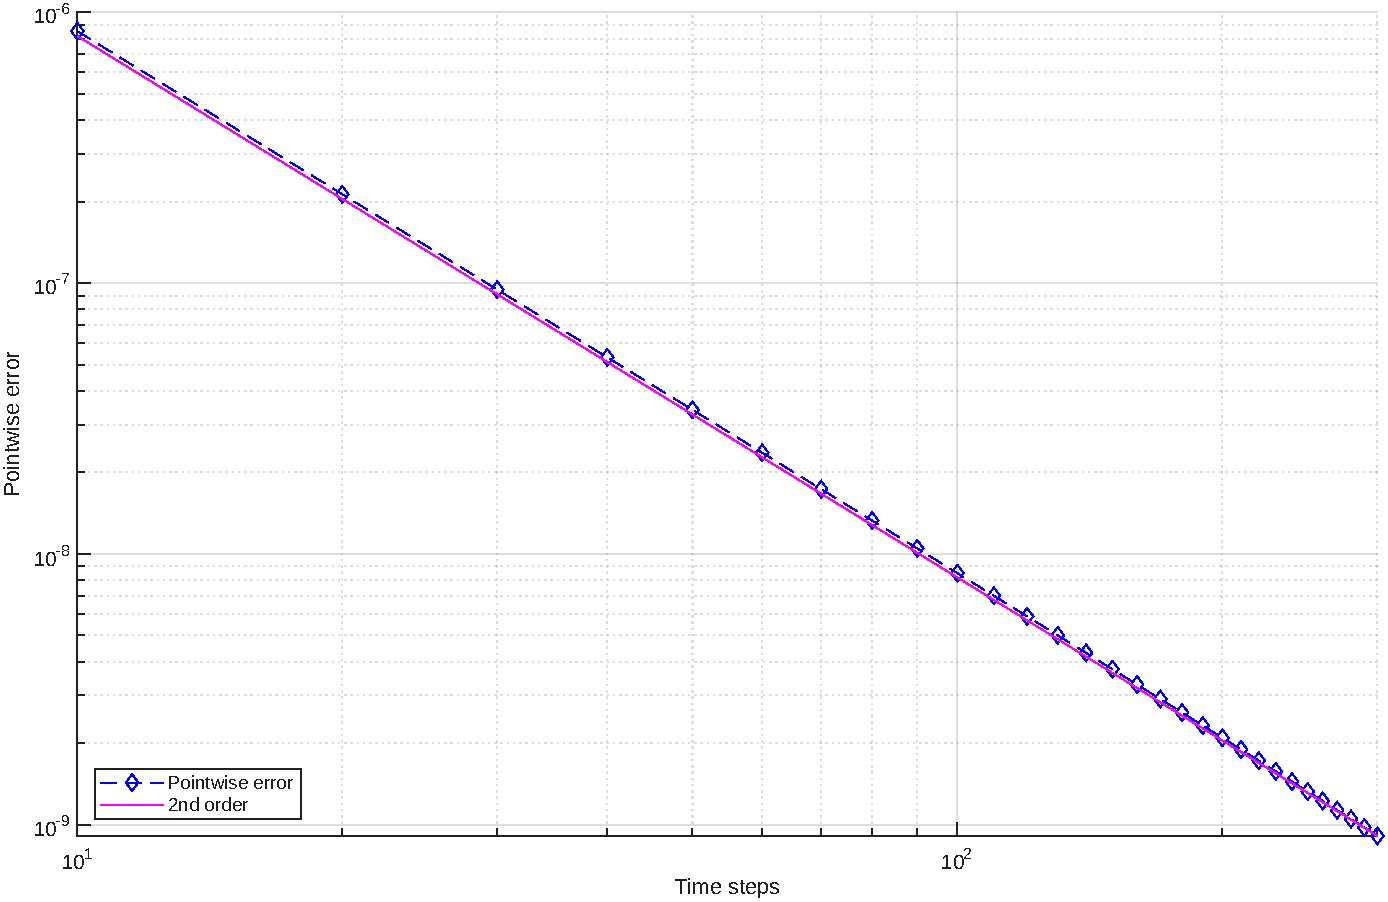
\includegraphics[width=0.8\textwidth]{img/time_conv.pdf}
    \caption{Convergence order}
\end{figure}


\subsection{Method applied to GPE}

In the case of GPE, we have $A = \frac\ii2 \lap$ and $B = \frac\ii2 \left(1 - \abs{u}^2\right)$. 

For $B$ we directly approximate the solution. The treatment for the first is more delicate: since in fact the Laplacian operator is approximated by the formula \ref{eq:lapprox}, we need to compute the matrix-vector product 

\[
    \exp\left(\frac\tau2 \left(I^y \kron D_2^x + D_2^y \kron I^x\right)\right)u_n
\]

which, for large matrices, is almost impossible dealing with in computationally reasonable times. Our goal would be avoiding the construction of any Kroneker product; instead we directly compute the action of the latter on the vector $\uu$. First we notice that $I^y \kron D_2^x$ and $D_2^y \kron I^x$ commute, as trivial consequence of the formula \ref{prop:prod}. This implies that 

\[ \exp\left(I^y \kron D_2^x + D_2^y \kron I^x\right) = \exp\left(I^y \kron D_2^x\right)\exp\left(D_2^y \kron I^x\right) \]

Since the exponential function is analytical, using \ref{th:analytic}, we have

\[ \exp\left(I^y \kron D_2^x\right) = I^y \kron \exp\left(D_2^x\right) \]

and the same for the other. Using again the formula \ref{prop:prod}, we obtain 

\[ \exp\left(I^y \kron D_2^x + D_2^y \kron I^x\right)\uu = \left(\exp\left(D_2^y\right) \kron \exp\left(D_2^x\right)\right)\uu \]

This is way better than directly compute the full exponential of Kroneker product, but it still requires the computation of a large full matrix. This can be avoided, since we can take into account the matrix $U = (u_{i,j}) \in \C^{m_x \times m_y}$, with the relation $U_{i,j} = u_{i + m_x(j - 1)}$, also denoted with $\mbox{Vec}(U) = u$. Let now $E_x = \exp\left(\tau D_2^x\right) = e_{i_1, j_1}$ and $E_y = \exp\left(\tau D_2^y\right) = e_{i_2, j_2}$. Thanks to \ref{prop:tensorprod}

